\section{Сбор информации}
Сбор информации является важной задачей в системах полнотекстового поиска, потому что именно качество собранной информации главным образом влияет на репрезентативность выборки, которую получит пользователь системы, совершающий запрос.

Данная задача порождает множество проблем, таких как: огромное количество заведомо нерелевантных страниц, ограничительная пропускная способность каналов, слабость серверов и пр.

В данном разделе приводится описание возникающих проблем и способы борьбы с ними.


\subsection{Архитектура робота}
Так или иначе архитектура любого поискового робота будет содержать некоторые общие для всех компоненты.

Упрощённо процесс работы такого робота состоит из следующих этапов (рис. \ref{fig:crawler}):
\begin{enumerate}
  \item Всё начинается с того, что пользователь роботом \framebox{1} добавляет в очередь \framebox{2} какой-то начальный набор адресов, с которого и начнётся обход;
  \item Загрузчик(и) страниц \framebox{3} получают из очереди \framebox{2} очередной адрес и производят соответствующий HTTP-запрос через сеть Интернет \framebox{4}. Чтобы избежать DNS-запросов перед загрузкой каждой страницы, часто кешируют IP-адрес домена;
  \item В случае успешного ответа загрузчик \framebox{3} передаёт страницу в экстрактор информации \framebox{4};
  \item Экстрактор информации \framebox{5} извлекает из страницы ссылки и полезную текстовую информацию. После чего ссылки добавляются в очередь \framebox{2}, а текстовой документ отправляется в индексатор \framebox{6};
  \item Индексатор \framebox{6} подготавливает документ и формирует запросы на сохранение в базу данных \framebox{7}.
\end{enumerate}

\begin{figure}[h]
  \centering
  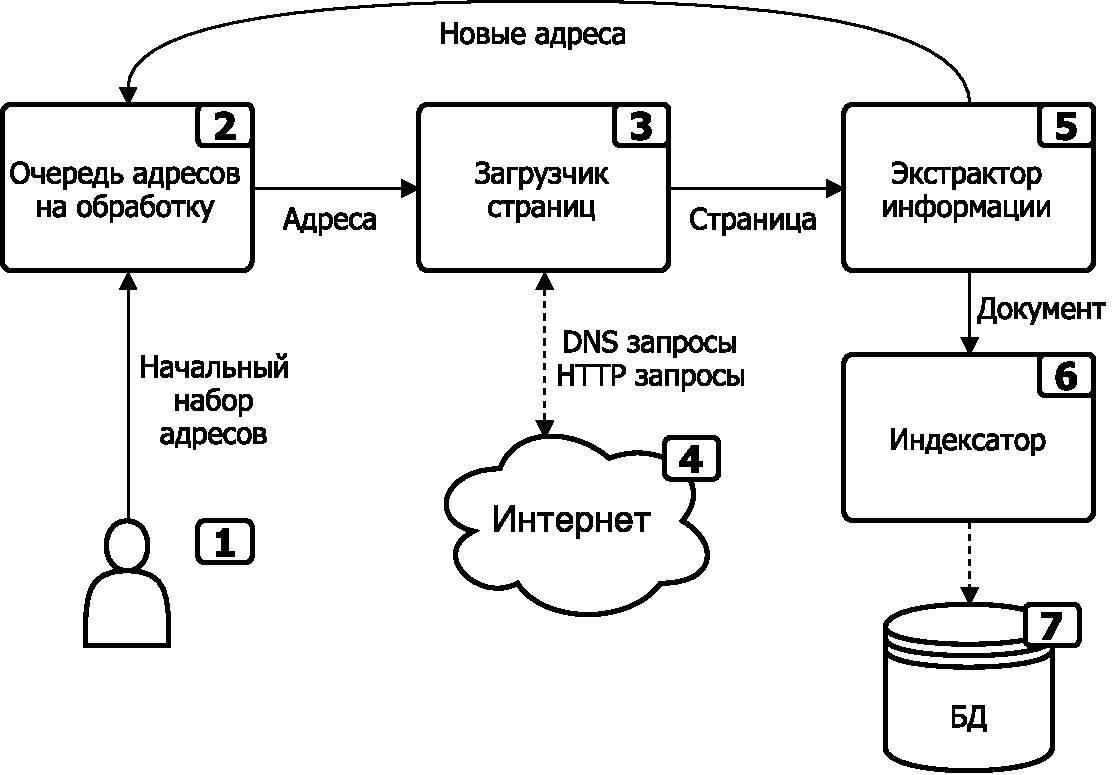
\includegraphics[width=\textwidth]{crawler.pdf}
  \caption{Типичная архитектура поискового робота.}
  \label{fig:crawler}
\end{figure}


\subsection{Фильтрация посещённых страниц}
Во время обхода важно отбрасывать ссылки, ведущие на страницы, которые уже были посещены или находятся в очереди на обработку. Очевидное на первый взгляд решение проблемы~--- использование ассоциативных массивов (причём скорее всего именно хеш-таблиц)~--- довольно требовательно к памяти.

Поэтому для фильтрации посещённых страниц применяется фильтр Блума.


\subsubsection{Фильтр Блума}
Фильтр Блума~--- вероятностная структура данных, позволяющая компактно хранить множество элементов и проверять принадлежность заданного элемента к множеству. При этом существует вероятность получить ложноположительный результат, то есть ситуацию, когда элемента в множестве нет, но фильтр сообщает, что элемент есть.

Фильтр Блума может использовать любой объём памяти, заранее заданный пользователем, причём чем он больше, тем меньше вероятность ложного срабатывания. Поддерживается операция добавления новых элементов в множество, но не удаления существующих (если только не используется модификация со счётчиками).

\begin{figure}[h]
  \centering
  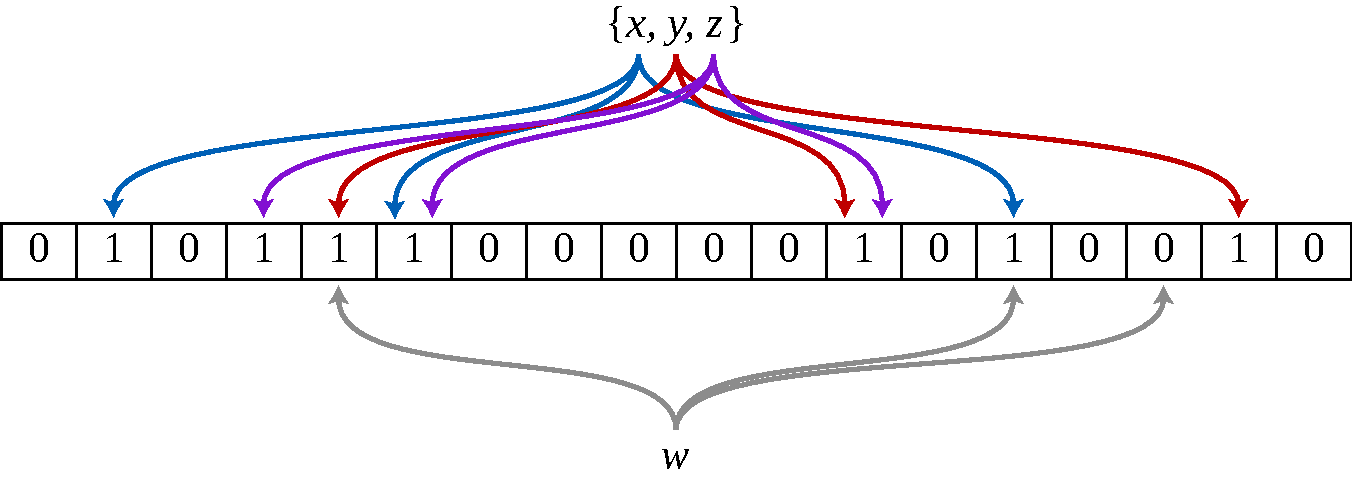
\includegraphics[width=\textwidth]{bloom-filter.pdf}
  \caption{Пример фильтра Блума с $m=18$ и $k=3$.}
\end{figure}

Фильтр Блума представляет собой битовый массив из $m$ бит. Изначально, когда структура данных хранит пустое множество, все $m$ бит обнулены. Пользователь должен определить $k$ независимых хеш-функций $h_i$, отображающих каждый элемент в одну из $m$ позиций битового массива достаточно равномерным образом.

Для добавления элемента $e$ необходимо записать единицы на каждую из позиций $h_i(e)$ битового массива.

Для проверки принадлежности элемента $e$ к множеству хранимых элементов, необходимо проверить состояние битов $h_i$. Если хотя бы один из них равен нулю, элемент не может принадлежать множеству (иначе бы при его добавлении все эти биты были установлены). Если все они равны единице, то структура данных сообщает, что $e$ принадлежит множеству. При этом может возникнуть две ситуации: либо элемент действительно принадлежит к множеству, либо все эти биты оказались установлены по случайности при добавлении других элементов, что и является источником ложных срабатываний в этой структуре данных.

Согласно \cite{broder02}, для заданных $n$~--- числа ожидаемых элементов в множестве и $p$~--- максимальной вероятности ложноположительного срабатывания возможно вычислить оптимальный размер $m$ как
\begin{equation}
  m=-\frac{n\ln p}{(\ln 2)^2},
\end{equation}
и оптимальное количество хеш-функций как
\begin{equation}
  k=\frac{m}{n}\ln 2.
\end{equation}


\subsubsection{Параметры фильтра Блума}
Количество максимально ожидаемых страниц очевидным образом зависит от глубины обхода:
\begin{equation}
  n=l^{d-1},
\end{equation}
\begin{conditions}
  $d$ & максимальная глубина обхода;\\
  $l$ & среднее количество ссылок на странице.
\end{conditions}

Так, при $l=100$, $d=4$ и $p=0.00001$ (ожидается не более одного ложноположительного срабатывания на 10 миллионов) потребуется всего $\approx 2.86$МБ данных.


\subsection{Стандарт исключений для роботов} \label{ssec:robotstxt}
Когда владельцы сайта хотят ограничить доступ к определённым страницам для поисковых ботов, они используют для этого файл \verb|robots.txt|, находящийся в корне сайта (то есть по пути \verb|/robots.txt|). Это может быть полезно для ограничения частоты запросов со стороны роботов, запрета индексирования динамический и служебных страниц.

Формат файла имеет следующий вид:
\begin{verbatim}
<поле>:<необязательный пробел><значение><необязательный пробел>
\end{verbatim}

Стоит заметить, что вместо пробела могут использоваться также другие пробельные символы, а \verb|поле| является регистронезависимым.

Основные используемые поля:
\begin{itemize}
  \item \verb|user-agent|: стандартное поле, используется для задания имени бота, которому адресованы последующие правила, либо \verb|*|, если всем;
  \item \verb|disallow|: стандартное поле, используется для задания пути, индексация которого запрещена. В пути разрешены два спец-символа: \verb|*| (любое количество любых символов) и \verb|$| (конец пути). Причём путь, к примеру, \verb|/path/to/file| действует аналогично \verb|/path/to/file*|;
  \item \verb|crawl-delay|: нестандартное поле, используется для задания минимальной задержки в секундах между запросами со стороны робота.
\end{itemize}


\subsection{Разбор страницы}
После загрузки страницы необходимо подготовить её к индексации~--- выделить полезную информацию: определить заголовок, слова для индексации, ссылки для загрузки.


\subsubsection{Декодирование мнемоник HTML}
Мнемоника~--- это конструкция SGML, которая ссылается на символ из набора символов текстового файла. В HTML предопределено большое количество спецсимволов. Чтобы вставить определённый символ в разметку, нужно вставить определенную ссылку-мнемонику в HTML-структуру.

Мнемоника имеет вид \verb|&...;|. Так, например, буква <<q>> может представляться как \verb|&#113;|, а <<--->> как \verb|&mdash;|.

Необходимость в декодировании символов-мнемоник исходит из нескольких причин:
\begin{enumerate}
  \item Мнемоники встречаются в заголовках страницы, который будет отображаться пользователю при поиске;
  \item Должны индексироваться не мнемоники, а только их значения. Так, мнемоника \verb|&empty;| (<<$\varnothing$>>) не должна индексироваться как слово <<empty>>.
\end{enumerate}


\subsubsection{Выделение содержимого} \label{sssec:readability}
Далеко не вся информация на странице ценна для поиска. Например, информация, размещённая в подвале и по сторонам страницы несёт обычно служебную информацию, которая может быть полезна при обходе страниц (так как может содержать полезные ссылки), но бесполезна конечному пользователю. Поэтому ставится вопрос об ограничении индексации исключительно полезными частями страницы. Для этого необходимы методы выделения такой информации, которые в основном базируются на эвристики и неплохо работают во многих случаях \cite{pomikalek11}.

Для получения основного содержимого во многих случаях достаточно сохранять только текстовые элементы HTML, то есть блоки текста, которые не прерывались разметкой, которые имеют более чем десяток слов. Люди выбираюсь один из двух типов текста для двух различных мотивов написания текста: <<навигационного>> и <<информационного>>.

Для элементов навигации обычно применяется текст, состоящий из нескольких слов (например, <<STOP>>, <<Прочтите это>>, <<Нажмите здесь>>), в то время как для основого содержимого используется много слов.

В то время как это разделение работает во множестве случаев, все становится сложнее с заголовками, короткими предложениями, отказами от ответственности, авторскими правами и другими колонтитулами.

Есть более сложные стратегии, а также функции, которые помогают отделять основное содержание от шаблонного \cite{kohlschutter10}:
\begin{enumerate}
  \item Рассмотренная выше плотность HTML-тегов;
  \item Ссылочная плотность (количество слов внутри ссылок по сравнению с общим количеством слов в блоке);
  \item Связь текущего блока с контекстом (с предыдущими и следующими блоками);
  \item DOM-структура документа (\verb|<article>|, \verb|<section>| и другие);
  \item Визуальное изображение страницы (например, большие изображения, окружённые текстом);
  \item Различные машинно-обученные алгоритмы.
\end{enumerate}

Результирующий алгоритм, используя комбинацию этих факторов, рекурсивно оценивает все узлы документа, находя наиболее похожие на основное содержимое.


\subsubsection{Выделение ссылок} \label{sssec:links}
Ссылки на странице могут быть обнаружены во многих местах: \verb|<a>|, \verb|<link>|, \verb|<script>| и др. Но для поискового бота по (x)html интерес представляют только ссылки в \verb|<a>|, причём далеко не все. Для уменьшения количества бесполезных запросов, связанных, например, с неиспользуемым языком, которые скорее всего всё равно будут выявлены на этапе получения заголовков (HTTP-заголовок \verb|content-language|), можно попробовать угадать по адресу ссылки релевантность.

Рассмотрим несколько методов фильтрации ссылок:
\begin{enumerate}
  \item По наличию букв из неиспользуемых алфавитов в пути ссылки. Действительно, если ссылка содержит несколько таких символов, то скорее всего представленная информация на странице имеет тот же язык;
  \item Использование чёрного или белого списков расширений, которые позволяет откидывать страницы с заведомо нерелевантной информацией, например \verb|.jpg|. Чёрный список задаётся списком запрещённых разрешений, в том время как белый список~--- разрешённых, например \verb|.html|, \verb|.asp| и \verb|.php|;
  \item Фильтрация доменов, так же основанная на чёрном или белом списках;
  \item Фильтрация поддоменов, основанная на некоторой эвристике. Например, поддомены \verb|git.| и \verb|svn.| часто содержат соответствующие репозитории, индексировать которые в большинстве случаев не имеет смысла.
\end{enumerate}


Кроме того, ссылки, заданные через \verb|<a>| могут иметь атрибут \verb|rel="nofollow"|, который используется для того, чтобы запретить учитывать данную ссылку поисковыми ботами при индексации страницы и передавать по ней вес данной страницы при расчёте PageRank. Чаще всего таким образом помечаются рекламные ссылки. Несмотря на то, что в индекс данные ссылки не попадают, включать их в оборот всё же имеет смысл.


\subsubsection{Стоп-слова}
Существование заведомо высокочастотных слов (таких как <<an>>, <<and>>, <<и>>, <<как>> и др.) ведёт к раздуванию индекса и, как следствие, замедлению работы поиска. При этом их вклад в ранжирование минимален. Поэтому разумно отказаться от индексирования таких слов вообще, путём занесения их в списки так называемых стоп-слов.


\subsubsection{Стемминг} \label{sssec:stemming}
Стемминг~---процесс нормализации слов путём выделения основы. Это позволяет учитывать морфологически близкие слова как формы одно и того же слова (например, <<connect>> и <<connected>> или <<чистый>> и <<чистая>>), что сильно улучшает ранжирование и упрощает поиск.

Наиболее известен алгоритм стемминга Портера. Алгоритм не использует баз основ слов, а работает, последовательно применяя ряд правил отсечения окончаний и суффиксов \cite{porter97}.

Рассмотрим версию алгоритма для русского языка \cite{porter06}.

Во-первых, в слове выделяются три зоны:
\begin{description}
  \item[RV] область слова после первой гласной. Может быть пустой, если гласных в слове нет;
  \item[R1] область слова после первого сочетания <<гласная-согласная>>;
  \item[R2] область R1 после первого сочетания <<гласная-согласная>>.
\end{description}

Далее выделяются группы окончаний слов:
\begin{itemize}
  \item Совершенного герундия (<<в>>, <<вши>>, <<вшись>> после <<а>> или <<я>>; <<ив>>, <<ивши>>, <<ившись>>, <<ыв>>, <<ывши>>, <<ывшись>>);
  \item Прилагательных (<<ее>>, <<ие>>, <<ые>>, <<ое>>, <<ими>>, <<ыми>>, <<ей>>, <<ий>>, <<ый>>, <<ой>>, <<ем>>, <<им>>, <<ым>>, <<ом>>, <<его>>, <<ого>>, <<ему>>, <<ому>>, <<их>>, <<ых>>, <<ую>>, <<юю>>, <<ая>>, <<яя>>, <<ою>>, <<ею>>);
  \item Причастных (<<eм>>, <<нн>>, <<вш>>, <<ющ>>, <<щ>> после а и я; <<ивш>>, <<ывш>>, <<ующ>>);
  \item Возвратных (<<ся>>, <<сь>>);
  \item Глагольных (<<ла>>, <<на>>, <<ете>>, <<йте>>, <<ли>>, <<й>>, <<л>>, <<ем>>, <<н>>, <<ло>>, <<но>>, <<ет>>, <<ют>>, <<ны>>, <<ть>>, <<ешь>>, <<нно>> после а или я; <<ила>>, <<ыла>>, <<ена>>, <<ейте>>, <<уйте>>, <<ите>>, <<или>>, <<ыли>>, <<ей>>, <<уй>>, <<ил>>, <<ыл>>, <<им>>, <<ым>>, <<ен>>, <<ило>>, <<ыло>>, <<ено>>, <<ят>>, <<ует>>, <<уют>>, <<ит>>, <<ыт>>, <<ены>>, <<ить>>, <<ыть>>, <<ишь>>, <<ую>>, <<ю>>);
  \item Существительных (<<а>>, <<ев>>, <<ов>>, <<ие>>, <<ье>>, <<е>>, <<иями>>, <<ями>>, <<ами>>, <<еи>>, <<ии>>, <<и>>, <<ией>>, <<ей>>, <<ой>>, <<ий>>, <<й>>, <<иям>>, <<ям>>, <<ием>>, <<ем>>, <<ам>>, <<ом>>, <<о>>, <<у>>, <<ах>>, <<иях>>, <<ях>>, <<ы>>, <<ь>>, <<ию>>, <<ью>>, <<ю>>, <<ия>>, <<ья>>, <<я>>);
  \item Превосходных (<<ейш>>, <<ейше>>);
  \item Словообразовательных (<<ост>>, <<ость>>);
  \item Адъективированных (определяется как прилагательное или причастие + прилагательное окончание).
\end{itemize}

При поиске окончания из всех возможных выбирается наиболее длинное. Например, в слове <<величие>> выбираем окончание <<ие>>, а не <<е>>.

Все проверки производятся над областью RV. Так, при проверке на совершенный герундий предшествующие буквы <<а>> и <<я>> также должны быть внутри RV. Буквы перед RV не участвуют в проверках вообще.

\begin{enumerate}
  \item Найти окончание совершенного герундия. Если оно существует~--- удалить его и завершить этот шаг. Иначе, удаляем возвратное окончание, если существует. Затем по порядку удаляется адъективированное окончание, глагольное окончание, окончание существительного. Как только одно из них найдено~--- шаг завершается;
  \item Если слово оканчивается на <<и>>~--- удалить <<и>>;
  \item Если в R2 найдётся словообразоваельное окончание~--- удалить его.
  \item Возможен один из трёх вариантов:
    \begin{enumerate}
      \item Если слово оканчивается на <<нн>>~--- удалить последнюю букву;
      \item Если слово оканчивается на превосходное окончание~--- удаляем его и снова проверяем <<нн>>;
      \item Если слово оканчивается на <<ь>>~--- удалить его.
    \end{enumerate}
\end{enumerate}

Аналогично существуют версии алгоритма для многих европейских языков, однако в данной работе используется только русский и английский языки.


\subsubsection{URL нормализация} \label{sssec:url-normalization}
Различные URL могут указывать на одну и ту же страницу, но отличаться при этом незначительно.

URL нормализация~--- процесс приведения URL к каноничному виду, путём применения различных правил трансляции адресов. Не все правила дают строго эквивалентные URL, однако на практике эти эвристики работают неплохо \cite{pant04}.

Ключ страницы~--- своего рода хеш, получаемый в результате агрессивной нормализации, то есть применения всех правил, указанных в данном разделе.

Относительно безопасные преобразования:
\begin{enumerate}
  \item Конвертация в нижний регистр компонентов схемы и хоста: \\ \verb|HTTP://www.Example.com/| в \verb|http://www.example.com/|;
  \item Удаление относительных каталогов, сегментов-точек: \\ \verb|http://example.com/../a/b/../c/./d| в \verb|http://example.com/a/c/d|;
  \item Удаление фрагментов: \\ \verb|http://example.com/bar.html#section1| в \verb|http://example.com/bar.html|;
  \item Удаление конечного слеша: \\ \verb|http://example.com/foo/| в \verb|https://example.com/foo|;
  \item Удаление порта по умолчанию: 80 для http и 443 для https \\ \verb|http://example.com:80| в \verb|http://example.com|;
  \item Перевод IDN в unicode: \\ \verb|http://xn--e1afmkfd.xn--80akhbyknj4f/| в \verb|http://пример.испытание/|.
\end{enumerate}

Преобразования, которые можно использовать для проверки эквивалентности двух страниц, но не при запросе:
\begin{enumerate}
  \item Удаление головного индекса (\verb|index.html|, \verb|default.aspx| и другие): \\ \verb|http://example.com/index.html| в \verb|http://www.example.com/|;
  \item Удаление дублированных слешей: \\ \verb|http://example.com/foo//bar.html| в \verb|http://example.com/foo/bar.html|;
  \item Удаление \verb|www.|: \\ \verb|http://www.example.com/| в \verb|http://example.com/|;
  \item Сокращение идентификаторов протокола: \\ \verb|https://example.com| в \verb|http://example.com|;
  \item Конвертация в нижний регистр всего URL: \\ \verb|HTTP://example.COM/TEST.html| в \verb|http://example.com/test.html|;
\end{enumerate}

Кроме того, так как для работы с динамическими страницами (их URL чаще всего содержат поисковую компоненту) требуется наличие отлаженного и надёжного метода определения дубликатов страницы, в данной работе было решено отказаться от подобных ссылок~--- к ссылке добавляется атрибут \verb|rel="nofollow"|, а запрос отбрасывается: \\ \verb|http://example.com/?id=123&q=test| в \verb|http://example.com/|.
